The block diagram for the inner loop is shown in Figure~\ref{fig:hw_ballbeam_PD_inner},
where 
\[
b_0 = \frac{\ell}{\frac{m_2\ell^2}{3}+m_1z_e^2}.
\]
\begin{figure}[H]
   \centering
   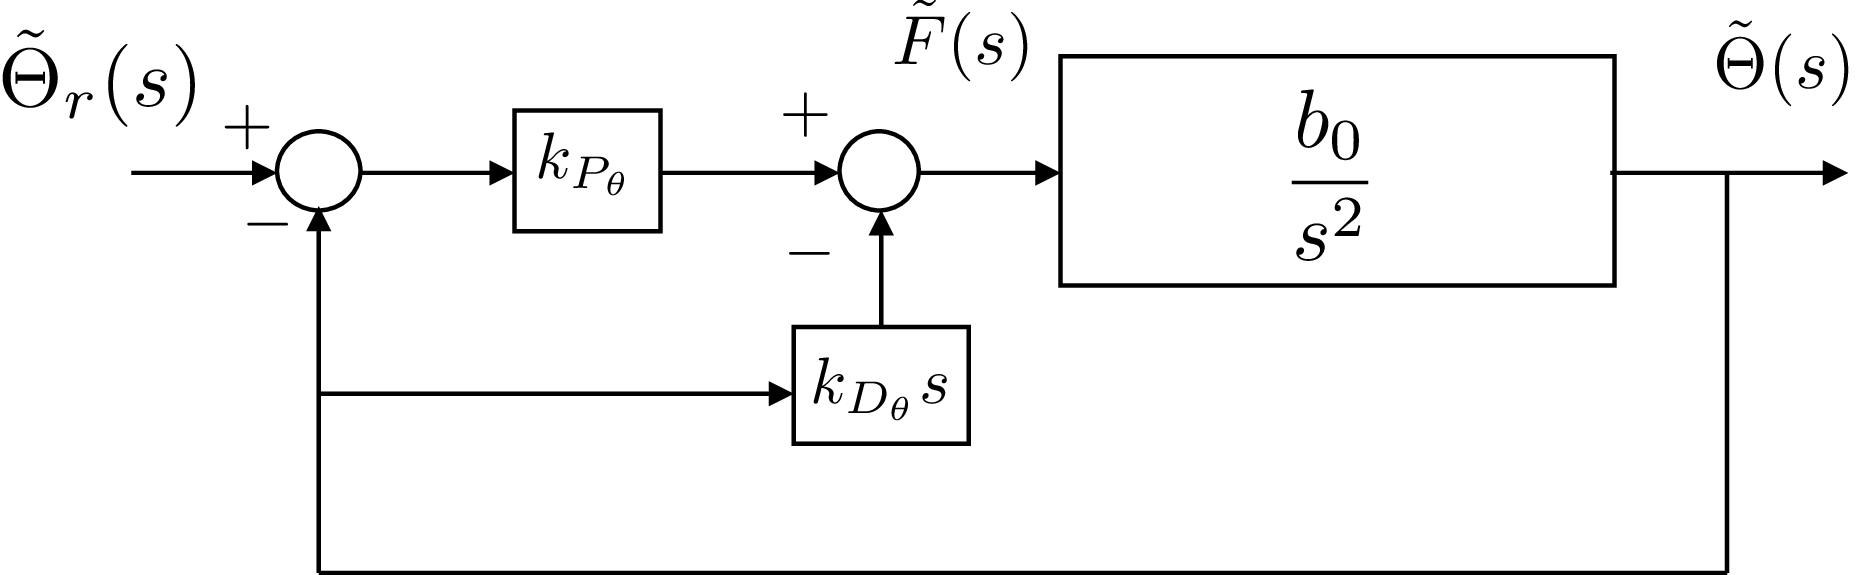
\includegraphics[width=0.8\textwidth]{6_design_studies/figures/hw_ballbeam_PD_inner.pdf}
   \caption{Block diagram for inner loop of the ball beam control.}
   \label{fig:hw_ballbeam_PD_inner}
\end{figure}

The closed loop transfer function from $\tilde{\Theta}_r$ to $\tilde{\Theta}$ is given by
\[
\tilde{\Theta}(s) = \frac{k_{P_\theta}b_0}{s^2+k_{D_\theta}b_0s+k_{P_\theta}b_0} \tilde{\Theta_r}(s).
\]
Therefore the closed loop characteristic equation is
\[
\Delta_{cl}(s) = s^2+k_{D_\theta}b_0s+k_{P_\theta}b_0.
\]
The desired closed loop characteristic equation is
\[
\Delta_{cl}^d(s) = s^2 + 2\zeta_{\theta}\omega_{n_\theta} s + \omega_{n_\theta}^2,
\]
where
\begin{align*}
\omega_{n_\theta} &= \frac{2.2}{t_{r_\theta}} = 2.2 \\
\zeta_{\theta} &= 0.707.
\end{align*}
Therefore
\begin{align*}
k_{P_\theta} &= \frac{w_{n_\theta}^2}{b_0} = 1.8251 \\
k_{D_\theta} &= \frac{2\zeta_{\theta}\omega_{n_\theta}}{b_0} = 1.1730.
\end{align*}
The DC gain of the inner loop is given by
\[
k_{DC_{\theta}} = \frac{k_{P_\theta}b_0}{k_{P_\theta}b_0} = 1.
\]

Replacing the inner loop by its DC gain, the block diagram for the outer loop is shown in Figure~\ref{fig:hw_ballbeam_PD_outer}.
\begin{figure}[H]
   \centering
   
\includegraphics[width=0.8\textwidth]{6_design_studies/figures/hw_ballbeam_PD_outer.pdf}
   \caption{Block diagram for outer loop of ball on beam closed loop system.}
   \label{fig:hw_ballbeam_PD_outer}
\end{figure}
The closed loop transfer function from $z_r$ to $z$ is given by
\[
Z(s) = \frac{-gk_{P_z}}{s^2-gk_{D_z}s-gk_{P_z}}Z_r(s).
\]
Note that the DC gain for the outer loop is equal to one.
The closed loop characteristic equation is therefore
\[
\Delta_{cl}(s) = s^2-gk_{D_z}s-gk_{P_z}.
\]
The desired characteristic equation is 
\[
\Delta_{cl}^d(s) = s^2 + 2\zeta_z\omega_{n_z}s + \omega_{n_z}^2,
\]
where
\begin{align*}
t_{r_z} &= 10 t_{r_\theta} = 10 \\
\omega_{n_z} &= \frac{2.2}{t_{r_z}} = 0.22 \\
\zeta_z &= 0.707.
\end{align*}
The PD gains are therefore
\begin{align*}
k_{P_z} &= -\frac{\omega_{n_z}^2}{g} = -0.0049 \\
k_{D_z} &= -\frac{2\zeta_z\omega_{n_z}}{g} = -0.0317.
\end{align*}

The Python, Matlab, and Simulink files are on the wiki page associated with the book.
